\documentclass[a4paper, 11pt, twocolumn]{article}
\usepackage[margin=0.8in]{geometry}
\usepackage{xcolor}
\usepackage{graphicx} %package to manage images
\graphicspath{ {./images/} }

\title{A2-08 Audio Systems}
\author{Revision sheet}
\date{}

\usepackage{fancyhdr}
\pagestyle{fancy}
\fancyhead{} % clear all header fields
\renewcommand{\headrulewidth}{0pt} % no line in header area
\fancyfoot{} % clear all footer fields
\renewcommand{\footrulewidth}{0.4pt}
\fancyfoot[C]{\thepage} % page number in centre of the page
\fancyfoot[R]{\footnotesize Thomas Boxall \\ Images from WJEC E-Book} % right hand footer has author name on top line and images reference on bottom line
\fancyfoot[L]{\footnotesize A2-08 Audio Systems \\ Revision sheet} % left hand footer has title of document on top line and 'Revision Sheet' on bottom line


\begin{document}
    
    \maketitle

    \section{Introduction}
    \thispagestyle{fancy}
    There are lots of different components which go into an audio system. The diagram shows a mono audio system.
    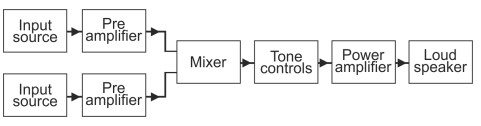
\includegraphics[width=0.4\textwidth]{monoBloc.jpg} \\
    \section{Input \& Pre-amp}
    A typical input would be a microphone. This produces a very small output so before the signal can be processed, it has to be amplified.
    \subsection{Signal transfer}
    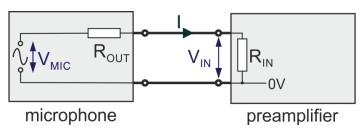
\includegraphics[width=0.4\textwidth]{sigTrans1.jpg} \\
    As there are two resistors drawn in series, this could also be shown as a potential divider.
    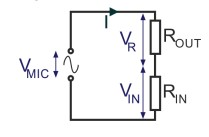
\includegraphics[width=0.4\textwidth]{sigTrans2.jpg} \\
    For maximum voltage transfer, we want $Rin>>Rout$, this should be about 10X greater.
    \subsection{Pre-amplifier}
    A multi-stage amplifier is usually used here. To maximise bandwidth, the stages need equal gain.
    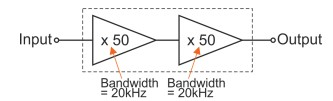
\includegraphics[width=0.4\textwidth]{msAmp.jpg} \\
    The gain and bandwidth can be calculated using the GBP equation
    $Gain Bandwidth Product = Gain \times Bandwith$
    \subsubsection{AC coupling}
    The op-amps used in the circuit amplify all frequencies, right down to 0Hz. We need to block these signals as they are DC signals and will break things further down the circuit. To do this, we use DC blocking coupling capacitors placed like so. \\
    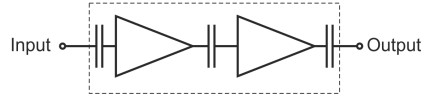
\includegraphics[width=0.4\textwidth]{dcBlock.jpg} \\
    The amplifier design is based off of a non-inverting amplifier with one added resistor to give the DC signals a path to ground. Below is one stage of a two-stage amp, you'd need to connect the output of one into the input of the next to get a two-stage amp. \\
    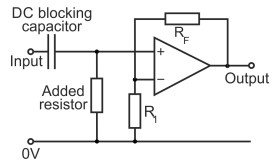
\includegraphics[width=0.4\textwidth]{singleStageAmp.jpg} \\

    \section{Audio Mixer}
    The audio mixer is based off of a Summing Amplifier.
    \subsection{Summing amplifier}
    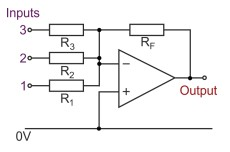
\includegraphics[width=0.4\textwidth]{summingAmp.jpg} \\
    $\displaystyle Vout = -R_f(\frac{V_1}{R_1} + \frac{V_2}{R_2} + \frac{V_3}{R_3})$ \\
    This basic design isn't great as you can't control the volume of each channel.

    \subsection{Adding gain control}
    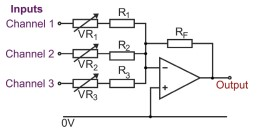
\includegraphics[width=0.4\textwidth]{summingAmpAddGain.jpg}\\
    Channel gain: $\displaystyle Ch. gain = \frac{-R_F}{F_1}$\\
    Minimum channel gain: $\displaystyle Min. ch. gain = \frac{-R_F}{VR+R}$\\
    Maximum channel gain: $\displaystyle Max. ch. gain = \frac{-R_F}{R}$\\
    There is a flaw with this design. The gain is always greater than 1 therefore you can't completely mute a channel (as this would require Gain=0). There a better design which fixes this.

    \subsection{Potentiometer design}
    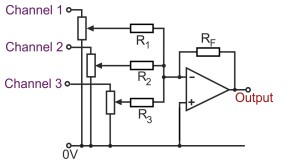
\includegraphics[width=0.4\textwidth]{potentAmp.jpg} \\
    As this design has potentiometers, we can change the ratio of resistors so 'all the voltage flows through the one which we aren't taking the output of', allowing us to set gain=0.

    \section{Tone Controls}
    Tone controls are designed using active filters. The main difference between active and passive filters is that active filters are built using an op-amp therefore their gain can exceed 1, allowing us to have boost filter.
    \subsection{Break Frequency}
    It is defined as the frequency at which the reactance of the capacitor is equal to the resistance of the resistor that is in the RC network.
    This can be calculated using the formula; $\displaystyle f_b = \frac{1}{2\Pi RC}$
    The formula is the same for all the types of active filter. It is important to choose the right resistor, which is the one 'touching' the capacitor.
    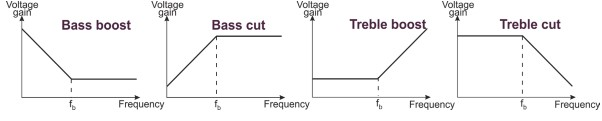
\includegraphics[width=0.45\textwidth]{activeFilterGraphs.jpg}
    \subsubsection{Bass Boost}
    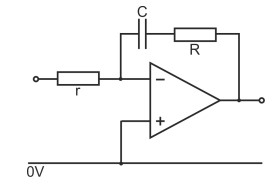
\includegraphics[width=0.4\textwidth]{bassBoost.jpg} \\
    Gain at high frequencies: $\displaystyle G = -\frac{R}{r}$
    \subsubsection{Bass Cut}
    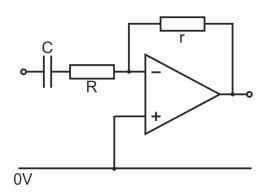
\includegraphics[width=0.4\textwidth]{bassCut.jpg} \\
    Gain at high frequencies: $\displaystyle G = -\frac{r}{R}$
    \subsubsection{Treble Boost}
    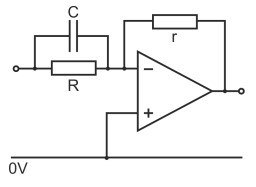
\includegraphics[width=0.4\textwidth]{trebleBoost.jpg} \\
    Gain at low frequencies: $\displaystyle G = -\frac{r}{R}$
    \subsubsection{Treble cut}
    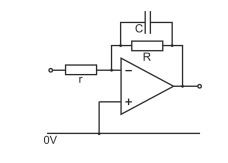
\includegraphics[width=0.4\textwidth]{trebleCut.jpg} \\
    Gain at low frequencies: $\displaystyle G = -\frac{R}{r}$

    \section{Power Amplifiers}
    This section also covers transfer to loudspeakers.\\
    Power Amplifiers are used to amplify the current of the output of the tone controls before the signal enters the loudspeaker.
    \subsection{Maximum Power Transfer theorem}
    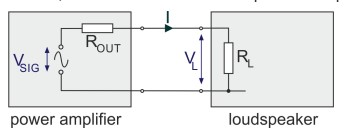
\includegraphics[width=0.4\textwidth]{paToLs.jpg}\\
    The maximum power is transferred when the resistance of the load is equal to the output resistance of the amplifier.
    \subsection{Emitter Follower}
    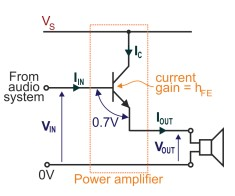
\includegraphics[width=0.4\textwidth]{emmitterFollower.jpg} \\
    Power in: $P_{in} = V_{in} \times I_B$\\
    Power out: $P_{out} = h_{FE} \times P_{in}$ \\
    Input Impedance: $\displaystyle R_{in} = \frac{V_{in}}{h_{FE}}$ \\
    Output Impedance: $\displaystyle R_{out} = \frac{R_{in}}{h_{FE}}$ \\
    The output impedance is much smaller than the input impedance therefore this an impedance buffer as it transforms the impedance. This matches the high output impedance of the tone controls to the low load impedance of a loudspeaker. \\
    There are a number of problems with this design which make it completely impractical to use.
    \begin{itemize}
        \item Not efficient
        \item Waste lots of power
        \item They have a region where nothing is amplified.
        \item Generally, they're terrible
    \end{itemize}
    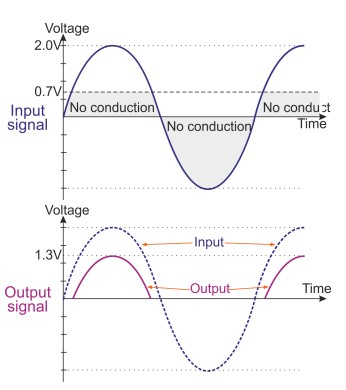
\includegraphics[width=0.4\textwidth]{issueWithEF.jpg}\\
    As the graph shows, everything below 0.7V is not amplified, and what is above it is reduced by 0.7V. To solve this, we need to add a DC voltage to Vin, this is done by biasing the amp.
    \subsection{Biased amplifier}
    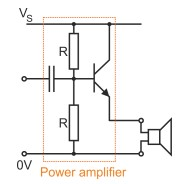
\includegraphics[width=0.4\textwidth]{biasedAmp.jpg}\\
    As the resistors are equal, Vs will be split into two, giving a bias voltage.\\
    $\displaystyle V_{bias} = \frac{V_s}{2}$\\
    $\displaystyle V_x = V_{in} + V_{bias}$ ($V_x$ is the voltage after the resistors) \\
    $V_{out} = V_x - 0.7$ \\
    This gives us a much better output
    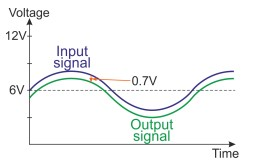
\includegraphics[width=0.4\textwidth]{biasOut.jpg} \\

    \subsection{Source Follower}
    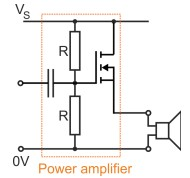
\includegraphics[width=0.4\textwidth]{sourceFollower.jpg}\\
    This type of amplifer has an advantage over the emitter follower due to its infinite input resistance.
    The MOSFET doesn't conduct until the input signal reaches 3V, hence the amplitude of the output is 3V smaller than the amplitude of the input. \\
    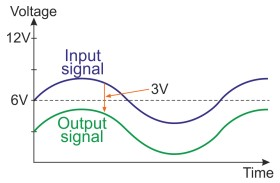
\includegraphics[width=0.4\textwidth]{sourceFollowerOut.jpg}\\
    A disadvantage of both the Source follower and the emitter follower is that the transistor is always conducting, even when there is no input signal - so it is always dissipating energy as heat.

    \subsection{Push-pull amplifiers}
    If we use a NPN transistor (the type we've been using already) and a PNP (the same as a NPN but reversed polarity) together, we can get an amplifier which will amplifier both positive and negative signals.\\
    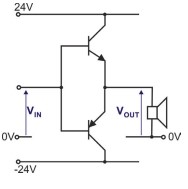
\includegraphics[width=0.4\textwidth]{pushPull.jpg}\\
    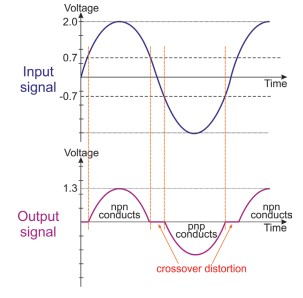
\includegraphics[width=0.4\textwidth]{pushPullOut.jpg} \\
    As seen on the graph, there is a region (between 0.7 and -0.7) where neither of the amplifiers conducts. This is called crossover distortion and it can be fixed by adding an op-amp to the circuit.

    \subsection{Improved Push-Pull amplifer}
    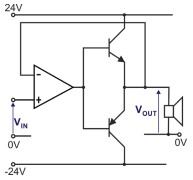
\includegraphics[width=0.4\textwidth]{opAmpPP.jpg}\\
    This solves the crossover distortion problem. This works by the op-amp trying to keep the inverting and non-inverting inputs at the same voltage, unless the output saturates. The inverting input is directly connected to the push-pull output and so the voltage at the output is always equal to the voltage at the non-inverting input, hence eliminating crossover distortion.

    \subsection{Maximising power output}
    $\displaystyle Max.P_{out} = P_{RMS_{MAX}} = \frac{V_s^2}{8R_L}$ where $V_s$ is the voltage between the rails.





\end{document}